\section{Descrizione dei singoli componenti}
\subsubsection{premi/client}
\begin{itemize}
  \item[] \textbf{Nome:}
  \item[] \textbf{Tipo:}
  \item[] \textbf{Package:} 
  \item[] \textbf{Descrizione:} 
  \item[] \textbf{Relazioni con altri componenti:} 
\end{itemize}


\subsection{premi/server}
\begin{figure}[h]
\begin{center}
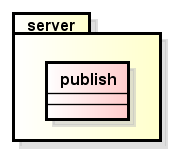
\includegraphics[scale=0.45]{img/diapkg/server.png}
\caption{Diagramma del package premi/server}
\end{center}
\end{figure}

\subsubsection{premi/server/publish}
\begin{itemize}
  \item[] \textbf{Nome:} publish
  \item[] \textbf{Tipo:} class
  \item[] \textbf{Package:} premi/server
  \item[] \textbf{Descrizione:} questa classe fornisce al lato client dell'applicazione dei metodi per l'inserimento, l'aggiornamento e la rimozione dei dati del database, e pubblica all'utente solo ed esclusivamente le informazioni a cui lui ha accesso
\end{itemize}






\subsection{premi/client}
\begin{figure}[h]
\begin{center}
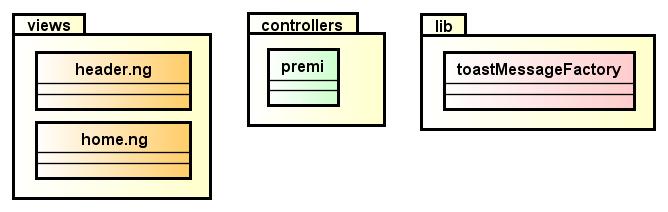
\includegraphics[scale=0.45]{img/diapkg/client.png}
\caption{Diagramma dei package views e controllers di premi}
\end{center}
\end{figure}


\subsubsection{premi/client/views/home.ng}
\begin{itemize}
  \item[] \textbf{Nome:} home.ng
  \item[] \textbf{Tipo:} template
  \item[] \textbf{Package:} premi/client/views
  \item[] \textbf{Descrizione:} template della pagina principale dell'applicazione
  \item[] \textbf{Relazioni con altri componenti:} la view generata da questo template è collegata allo \textit{\$scope} di premi/client/controllers/homeCtrl per l'aggiornamento in tempo reale dei dati visualizzati e modificati
\end{itemize}

\subsubsection{premi/client/views/info.ng}
\begin{itemize}
  \item[] \textbf{Nome:} info.ng
  \item[] \textbf{Tipo:} template
  \item[] \textbf{Package:} premi/client/views
  \item[] \textbf{Descrizione:} template della view che mostra all'utente informazioni sull'applicazione nella pagina principale
  \item[] \textbf{Relazioni con altri componenti:} la view generata da questo template è collegata allo \textit{\$scope} di premi/client/controllers/infoCtrl per l'aggiornamento in tempo reale dei dati visualizzati e modificati 
\end{itemize}


\subsubsection{premi/client/views/view.ng}
\begin{itemize}
  \item[] \textbf{Nome:} view.ng
  \item[] \textbf{Tipo:} template
  \item[] \textbf{Package:} premi/client/views
  \item[] \textbf{Descrizione:} template della view di supporto all'header della pagina principale dell'applicazione
  \item[] \textbf{Relazioni con altri componenti:} la view generata da questo template è collegata allo \textit{\$scope} di premi/client/controllers/premi per la gestione dell'header
\end{itemize}


\subsubsection{premi/client/views/container.ng}
\begin{itemize}
  \item[] \textbf{Nome:} container.ng
  \item[] \textbf{Tipo:} template
  \item[] \textbf{Package:} premi/client/views
  \item[] \textbf{Descrizione:} template "contenitore" di supporto ad altre viste
\end{itemize}
  
  
\subsubsection{premi/client/views/fluidContainer.ng}
\begin{itemize}
  \item[] \textbf{Nome:} fluidContainer.ng
  \item[] \textbf{Tipo:} template
  \item[] \textbf{Package:} premi/client/views
  \item[] \textbf{Descrizione:} template "contenitore" di supporto ad altre viste
\end{itemize}


\subsubsection{premi/client/controllers/homeCtrl}
\begin{itemize}
  \item[] \textbf{Nome:} homeCtrl
  \item[] \textbf{Tipo:} controller
  \item[] \textbf{Package:} premi/client/controllers
  \item[] \textbf{Descrizione:} controller di premi/client/views/home.ng
   \item[] \textbf{Relazioni con altri componenti:} modella lo \textit{\$scope} per interagire con la view generata da premi/client/views/home.ng
\end{itemize}


\subsubsection{premi/client/controllers/infoCtrl}
\begin{itemize}
  \item[] \textbf{Nome:} infoCtrl
  \item[] \textbf{Tipo:} controller
  \item[] \textbf{Package:} premi/client/controllers
  \item[] \textbf{Descrizione:} controller di premi/client/views/info.ng
  \item[] \textbf{Relazioni con altri componenti:} modella lo \textit{\$scope} per interagire con la view generata da premi/client/views/info.ng 
\end{itemize}

\subsubsection{premi/client/controllers/premi}
\begin{itemize}
  \item[] \textbf{Nome:} premi
  \item[] \textbf{Tipo:} controller
  \item[] \textbf{Package:} premi/client/controllers
  \item[] \textbf{Descrizione:} controller di premi/client/views/view.ng
  \item[] \textbf{Relazioni con altri componenti:} modella lo \textit{\$scope} per interagire con la view generata da premi/client/views/info.ng e dipende anche da:
 \begin{itemize}
 \item \textit{premi/client/header/lib/Header} per la gestione dell'header della pagina principale
 \end{itemize}
\end{itemize}



\subsection{premi/client/header}

\begin{figure}[h]
\begin{center}
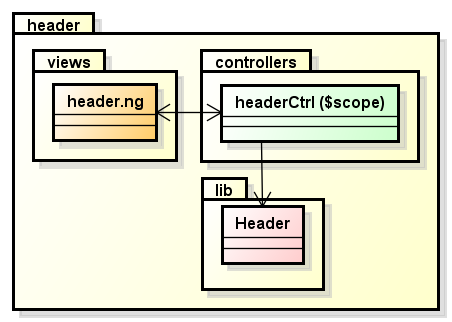
\includegraphics[scale=0.45]{img/diapkg/header.png}
\caption{Diagramma del package premi/client/header}
\end{center}
\end{figure}

\subsubsection{premi/client/header/views/header.ng}
\begin{itemize}
  \item[] \textbf{Nome:} header.ng
  \item[] \textbf{Tipo:} template
  \item[] \textbf{Package:} premi/client/header/views
  \item[] \textbf{Descrizione:} template dell'header della pagina principale dell'applicazione
  \item[] \textbf{Relazioni con altri componenti:} a view generata da questo template è collegata allo \textit{\$scope} di premi/client/header/controllers/headerCtrl per l'aggiornamento in tempo reale dell'header
\end{itemize}


\subsubsection{premi/client/header/controllers/headerCtrl}
\begin{itemize}
  \item[] \textbf{Nome:} headerCtrl
  \item[] \textbf{Tipo:} controller
  \item[] \textbf{Package:} premi/client/header/controllers
  \item[] \textbf{Descrizione:} controller di premi/client/header/views/header.ng
  \item[] \textbf{Relazioni con altri componenti:} modella lo \textit{\$scope} per interagire con la view generata da premi/client/header/views/header.ng e dipende anche da:
 \begin{itemize}
 \item \textit{premi/client/header/lib/Header} per la creazione dell'header della pagina principale
 \end{itemize}
\end{itemize}


\subsubsection{premi/client/header/lib/Header}
\begin{itemize}
  \item[] \textbf{Nome:} Header
  \item[] \textbf{Tipo:} class
  \item[] \textbf{Package:} premi/client/header/lib
  \item[] \textbf{Descrizione:} classe dell'header della pagina principale di Premi. Fornisce dei metodi per gestire la propria visualizzazione e per quella dello username, dello stato dell'applicazione e della barra di navigazione
\end{itemize} 




\subsection{premi/client/presentation}
\begin{figure}[!h]
\begin{center}
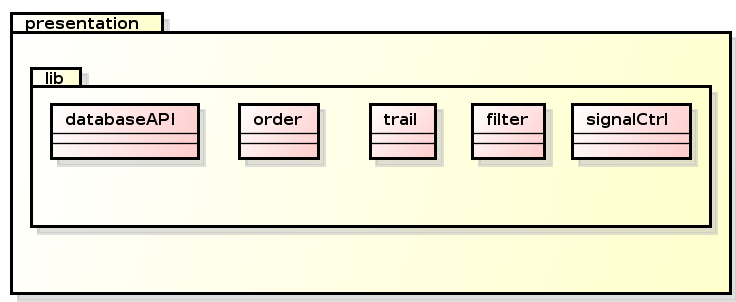
\includegraphics[scale=0.45]{img/diapkg/presentation.png}
\caption{Diagramma del package premi/client/presentation}
\end{center}
\end{figure}


\subsubsection{premi/client/presentation/lib/databaseAPI}
\begin{itemize}
  \item[] \textbf{Nome:} databaseAPI
  \item[] \textbf{Tipo:} class
  \item[] \textbf{Package:} premi/client/presentation/lib/
  \item[] \textbf{Descrizione:} estende i metodi di premi/server/publish e li specializza per i bisogni del client
   \item[] \textbf{Relazioni con altri componenti:} dipende da:
 \begin{itemize}
 \item \textit{premi/server/publish} per derivare i metodi di gestione dei dati lato client
 \end{itemize}
\end{itemize}


\subsubsection{premi/client/presentation/lib/OrderedGOList}
\begin{itemize}
  \item[] \textbf{Nome:} OrderedGoList
  \item[] \textbf{Tipo:} class
  \item[] \textbf{Package:} premi/client/presentation/lib/
  \item[] \textbf{Descrizione:} classe che modella una lista ordinata di oggetti grafici
\end{itemize}
  
\subsubsection{premi/client/presentation/lib/Trail}
\begin{itemize}
  \item[] \textbf{Nome:} Trail
  \item[] \textbf{Tipo:} class
  \item[] \textbf{Package:} premi/client/presentation/lib/
  \item[] \textbf{Descrizione:} classe che modella un Trail, ossia un percorso di presentazione. Deve poter fornire i metodi per scorrere la presentazione e inserire o rimuovere Frame e checkpoint
\end{itemize}



\subsection{premi/client/presentationManager}
\begin{figure}[!h]
\begin{center}
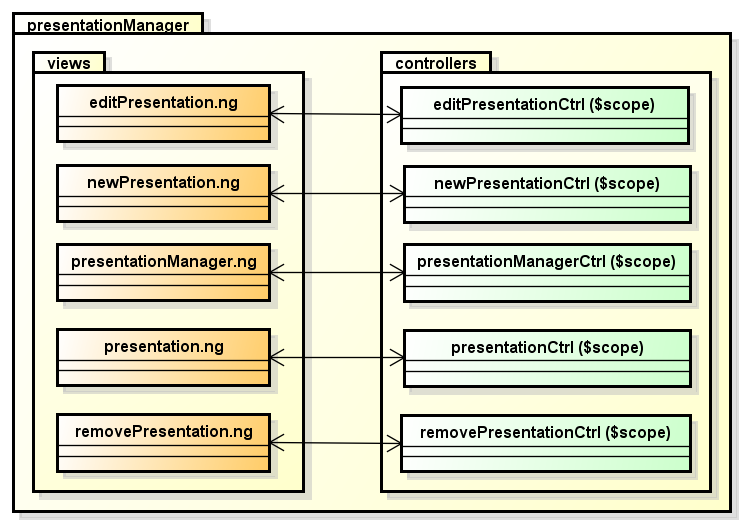
\includegraphics[scale=0.45]{img/diapkg/presentationManager.png}
\caption{Diagramma del package premi/client/presentation}
\end{center}
\end{figure}


\subsubsection{premi/client/presentationManager/views/editPresentation.ng}
\begin{itemize}
  \item[] \textbf{Nome:} editPresentation.ng
  \item[] \textbf{Tipo:} template
  \item[] \textbf{Package:}  premi/client/presentationManager/views/
  \item[] \textbf{Descrizione:} template della parte di pagina che offre all'utente la possibilità di modificare una presentazione
  \item[] \textbf{Relazioni con altri componenti:}  la view generata da questo template è collegata allo \textit{\$scope} di premi/client/presentationManager/controllers/editPresentationCtrl per la modifica di una presentazione
\end{itemize}

\subsubsection{premi/client/presentationManager/views/newPresentation.ng}
\begin{itemize}
  \item[] \textbf{Nome:} newPresentation.ng
  \item[] \textbf{Tipo:} template
  \item[] \textbf{Package:} premi/client/presentationManager/views/
  \item[] \textbf{Descrizione:} template della parte di pagina che offre all'utente la possibilità di creare una nuova presentazione
  \item[] \textbf{Relazioni con altri componenti:}  la view generata da questo template è collegata allo \textit{\$scope} di premi/client/presentationManager/controllers/newPresentationCtrl per l'aggiunta di una presentazione vuota nel database di proprietà dell'utente
\end{itemize}

\subsubsection{premi/client/presentationManager/views/presentationManager.ng}
\begin{itemize}
  \item[] \textbf{Nome:} presentationManager.ng
  \item[] \textbf{Tipo:} template
  \item[] \textbf{Package:} premi/client/presentationManager/views/
  \item[] \textbf{Descrizione:} template dello scheletro della pagina di gestione delle presentazioni dell'utente
  \item[] \textbf{Relazioni con altri componenti:}  la view generata da questo template è collegata allo \textit{\$scope} di premi/client/presentationManager/controllers/newPresentationCtrl
\end{itemize}

\subsubsection{premi/client/presentationManager/views/presentations.ng}
\begin{itemize}
  \item[] \textbf{Nome:} presentations.ng
  \item[] \textbf{Tipo:} template
  \item[] \textbf{Package:} premi/client/presentationManager/views/
  \item[] \textbf{Descrizione:} template della parte di pagina che mostra all'utente la lista delle sue presentazioni
  \item[] \textbf{Relazioni con altri componenti:} la view generata da questo template è collegata allo \textit{\$scope} di premi/client/presentationManager/controllers/presentationsCtrl per accedere alla lista delle presentazioni
\end{itemize}

\subsubsection{premi/client/presentationManager/views/removePresentation.ng}
\begin{itemize}
  \item[] \textbf{Nome:} removePresentation.ng
  \item[] \textbf{Tipo:} template 
  \item[] \textbf{Package:} premi/client/presentationManager/views/
  \item[] \textbf{Descrizione:} template della parte di pagina che offre all'utente la possibilità di eliminare una presentazione 
  \item[] \textbf{Relazioni con altri componenti:} la view generata da questo template è collegata allo \textit{\$scope} di premi/client/presentationManager/controllers/removePresentationCtrl per rimuovere una presentazione dal database
\end{itemize}

\subsection{Premi/client/frameEditor}
\begin{figure}[!h]
\begin{center}
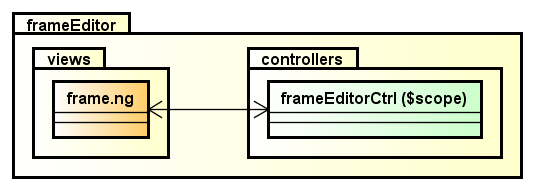
\includegraphics[scale=0.45]{img/diapkg/frameEditor.png}
\caption{Diagramma del package premi/client/frameEditor}
\end{center}
\end{figure}
\subsubsection{Premi/client/frameEditor/views/frame.ng}
\begin{itemize}
  \item[] \textbf{Nome:} frame.ng
  \item[] \textbf{Tipo:} class
  \item[] \textbf{Package:} Premi/client/frameEditor/views
  \item[] \textbf{Descrizione:} template della parte di pagina che permette la modifica dei Frame$_G$ e degli oggetti in esso contenuti.
\end{itemize}
\subsubsection{Premi/client/frameEditor/views/toolbar.ng}
\begin{itemize}
  \item[] \textbf{Nome:} toolbar.ng
  \item[] \textbf{Tipo:} class
  \item[] \textbf{Package:} Premi/client/frameEditor/views
  \item[] \textbf{Descrizione:} template della parte di pagina che mostra la toolbar che contiene tutte le funzionalità disponibili per la modifica di un frame e degli oggetti in esso contenuti.
\end{itemize}
\subsubsection{Premi/client/frameEditor/controllers/frameEditorCtrl}
\begin{itemize}
  \item[] \textbf{Nome:} FrameEditorCtrl
  \item[] \textbf{Tipo:} class
  \item[] \textbf{Package:} Premi/client/frameEditor/controllers
  \item[] \textbf{Descrizione:} controller di premi/client/frameEditor/views/toolbar.ng e di premi/client/frameEditor/views/frame.ng
  \item[] \textbf{Relazioni con altri componenti:} modella lo \textit{\$scope} per interagire con le views generate da premi/client/frameEditor/views/toolbar.ng e premi/client/frameEditor/views/frame.ng dipende anche da:
 \begin{itemize} 
	\item \textit{Premi/client/presentation/lib/databaseAPI} per interagire con il database;  
	\item \textit{Premi/client/editor/lib/interactInit} per interagire con la libreria Interactjs;
	\item \textit{Premi/client/editor/lib/frame} per interagire con la libreria frame e usare i metodi per la modifica, aggiunta, cancellazione di un frame;
	\item \textit{Premi/client/editor/lib/Observer} per interagire con la libreria observer; 
	\item \textit{Premi/presentation/lib/orderedGOList} per interagire con la libreria orderedGOList per ordinare la lista dei frame. 
  \end{itemize} 
\end{itemize}

\clearpage
\subsection{Premi/client/infographicEditor}
\begin{figure}[!h]
\begin{center}
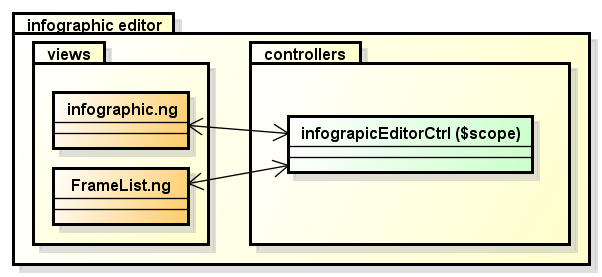
\includegraphics[scale=0.45]{img/diapkg/infographicEditor.png}
\caption{Diagramma del package premi/client/infographicEditor}
\end{center}
\end{figure}
\subsubsection{Premi/client/infographicEditor/views/infographic.ng}
\begin{itemize}
  \item[] \textbf{Nome:} infographic.ng
  \item[] \textbf{Tipo:} class
  \item[] \textbf{Package:} Premi/client/infographicEditor/views
  \item[] \textbf{Descrizione:}  template della parte di pagina per la creazione o modifica dell'infografica$_G$
\end{itemize}
\subsubsection{Premi/client/infographicEditor/views/frameList.ng}
\begin{itemize}
  \item[] \textbf{Nome:} frameList.ng
  \item[] \textbf{Tipo:} class
  \item[] \textbf{Package:} Premi.client.InfographicEditor.views
  \item[] \textbf{Descrizione:} template della parte di pagina che mostra la lista dei frame creati che possono essere inseriti nell'infografica.
\end{itemize}
\subsubsection{Premi/client/infographicEditor/controllers/infographicEditorCtrl}
\begin{itemize}
  \item[] \textbf{Nome:} infographicEditorCtrl
  \item[] \textbf{Tipo:} class
  \item[] \textbf{Package:} Premi/client/infographicEditor/controllers
  \item[] \textbf{Descrizione:} controller di premi/client/infographicEditor/views/frameList.ng e premi/client/infographicEditor/views/infographic.ng
  \item[] \textbf{Relazioni con altri componenti:} modella lo \textit{\$scope} per interagire con le views generate da Premi.client.InfographicEditor.views.frame.ng e di Premi.client.InfographicEditor.views.toolbar.ng e dipende da: 
  \begin{itemize}  
  \item[] \textit{Premi/client/presentation/lib/databaseAPI} per interagire con il database;
  \item[] \textit{Premi/client/editor/lib/interactInit} per interagire con la libreria interactjs;
  \item[] \textit{Premi/client/editor/lib/infographic} per interagire con la libreria infografica e usare i metodi per la gestione dell'infografica;
  \item[] \textit{Premi/client/editor/lib/observer} per interagire con la libreria observer;
  \item[] \textit{Premi/presentation/lib/orderedGOList} per interagire con la libreria orderedGOList per ordinare la lista dei frame. 
  \end{itemize}
\end{itemize}



\subsubsection{premi/client}
\begin{itemize}
  \item[] \textbf{Nome:}
  \item[] \textbf{Tipo:}
  \item[] \textbf{Package:} 
  \item[] \textbf{Descrizione:} 
  \item[] \textbf{Relazioni con altri componenti:} 
\end{itemize}

\subsubsection{premi/client}
\begin{itemize}
  \item[] \textbf{Nome:}
  \item[] \textbf{Tipo:}
  \item[] \textbf{Package:} 
  \item[] \textbf{Descrizione:} 
  \item[] \textbf{Relazioni con altri componenti:} 
\end{itemize}

\subsubsection{premi/client}
\begin{itemize}
  \item[] \textbf{Nome:}
  \item[] \textbf{Tipo:}
  \item[] \textbf{Package:} 
  \item[] \textbf{Descrizione:} 
  \item[] \textbf{Relazioni con altri componenti:} 
\end{itemize}

\subsubsection{premi/client}
\begin{itemize}
  \item[] \textbf{Nome:}
  \item[] \textbf{Tipo:}
  \item[] \textbf{Package:} 
  \item[] \textbf{Descrizione:} 
  \item[] \textbf{Relazioni con altri componenti:} 
\end{itemize}

\subsubsection{premi/client}
\begin{itemize}
  \item[] \textbf{Nome:}
  \item[] \textbf{Tipo:}
  \item[] \textbf{Package:} 
  \item[] \textbf{Descrizione:} 
  \item[] \textbf{Relazioni con altri componenti:} 
\end{itemize}

\subsubsection{premi/client}
\begin{itemize}
  \item[] \textbf{Nome:}
  \item[] \textbf{Tipo:}
  \item[] \textbf{Package:} 
  \item[] \textbf{Descrizione:} 
  \item[] \textbf{Relazioni con altri componenti:} 
\end{itemize}

\subsubsection{premi/client}
\begin{itemize}
  \item[] \textbf{Nome:}
  \item[] \textbf{Tipo:}
  \item[] \textbf{Package:} 
  \item[] \textbf{Descrizione:} 
  \item[] \textbf{Relazioni con altri componenti:} 
\end{itemize}



















